\documentclass[bachelor, och, pract]{SCWorks}
% параметр - тип обучения - одно из значений:
%    spec     - специальность
%    bachelor - бакалавриат (по умолчанию)
%    master   - магистратура
% параметр - форма обучения - одно из значений:
%    och   - очное (по умолчанию)
%    zaoch - заочное
% параметр - тип работы - одно из значений:
%    referat    - реферат
%    coursework - курсовая работа (по умолчанию)
%    diploma    - дипломная работа
%    pract      - отчет по практике
%    pract      - отчет о научно-исследовательской работе
%    autoref    - автореферат выпускной работы
%    assignment - задание на выпускную квалификационную работу
%    review     - отзыв руководителя
%    critique   - рецензия на выпускную работу
% параметр - включение шрифта
%    times    - включение шрифта Times New Roman (если установлен)
%               по умолчанию выключен
\usepackage[T2A]{fontenc}
\usepackage[utf8]{inputenc}
\usepackage{graphicx}

\usepackage[sort,compress]{cite}
\usepackage{amsmath}
\usepackage{amssymb}
\usepackage{amsthm}
\usepackage{fancyvrb}
\usepackage{longtable}
\usepackage{array}
\usepackage[english,russian]{babel}

\usepackage{inconsolata}

\usepackage{color}

\definecolor{pblue}{rgb}{0.13,0.13,1}
\definecolor{pgreen}{rgb}{0,0.5,0}
\definecolor{pred}{rgb}{0.9,0,0}
\definecolor{pgrey}{rgb}{0.46,0.45,0.48}

\usepackage{listings}
\lstset{language=Java,
  showspaces=false,
  showtabs=false,
  breaklines=true,
  showstringspaces=false,
  breakatwhitespace=true,
  commentstyle=\color{pgreen},
  keywordstyle=\color{pblue},
  stringstyle=\color{pred},
  basicstyle=\small,
  %moredelim=[il][\textcolor{pgrey}]{$$},
  moredelim=[is][\textcolor{pgrey}]{\%\%}{\%\%}
}

% Используется автором репозитория
%\usemintedstyle{xcode}
% Этот пакет включает в себя аналогичный Times New Roman шрифт.
% Необходим для успешной компиляции для UNIX-систем ввиду отсутствия TNR в нем.
% Можно использовать и для Windows.
\usepackage{tempora}


\usepackage[colorlinks=false]{hyperref}


\newcommand{\eqdef}{\stackrel {\rm def}{=}}

\newtheorem{lem}{Лемма}

% % При использовании biblatex вместо bibtex
%\usepackage[style=gost-numeric]{biblatex}
%\addbibresource{thesis.bib}

\begin{document}

% Кафедра (в родительном падеже)
\chair{информатики и программирования}

% Тема работы
\title{реализация консольного приложения для работы с графами}

% Курс
\course{3}

% Группа
\group{351}

% Факультет (в родительном падеже) (по умолчанию "факультета КНиИТ")
\department{факультета КНиИТ}

% Специальность/направление код - наименование
%\napravlenie{02.03.02 "--- Фундаментальная информатика и информационные технологии}
%\napravlenie{02.03.01 "--- Математическое обеспечение и администрирование информационных систем}
%\napravlenie{09.03.01 "--- Информатика и вычислительная техника}
\napravlenie{09.03.04 "--- Программная инженерия}
%\napravlenie{10.05.01 "--- Компьютерная безопасность}

% Для студентки. Для работы студента следующая команда не нужна.
%\studenttitle{Студентки}

% Фамилия, имя, отчество в родительном падеже
\author{Кондрашова Даиила Владиславовича}

% Заведующий кафедрой
\chtitle{доцент, к.\,ф.-м.\,н.} % степень, звание
\chname{М.\,В.\,Огнёва}

%Научный руководитель (для реферата преподаватель проверяющий работу)
\satitle{доцент, к.\,п.\,н.} %должность, степень, звание
\saname{А.\,П.\,Грецова}

% Руководитель практики от организации (только для практики,
% для остальных типов работ не используется)
%\patitle{к.\,ф.-м.\,н., доцент}
%\paname{Д.\,Ю.\,Петров}

% Семестр (только для практики, для остальных
% типов работ не используется)
\term{5}

% Наименование практики (только для практики, для остальных
% типов работ не используется)
\practtype{учебная}

% Продолжительность практики (количество недель) (только для практики,
% для остальных типов работ не используется)
\duration{16}

% Даты начала и окончания практики (только для практики, для остальных
% типов работ не используется)
\practStart{01.10.202023}
\practFinish{25.12.2023}

% Год выполнения отчета
\date{2023}

\maketitle

% Включение нумерации рисунков, формул и таблиц по разделам
% (по умолчанию - нумерация сквозная)
% (допускается оба вида нумерации)
%\secNumbering


\tableofcontents

% Раздел "Обозначения и сокращения". Может отсутствовать в работе
% \abbreviations
% \begin{description}
%     \item ... "--- ...
%     \item ... "--- ...
% \end{description}

% Раздел "Определения". Может отсутствовать в работе
%\definitions

% Раздел "Определения, обозначения и сокращения". Может отсутствовать в работе.
% Если присутствует, то заменяет собой разделы "Обозначения и сокращения" и "Определения"
%\defabbr


% Раздел "Введение"

%\intro

% После введения — серии \section, \subsection и т.д.

\section{Определение графа пользователем и в программе}

\subsection{Определение графа пользователем}

Предполагается, что пользователь будет задавать граф в следующем виде:
\bigskip

Пусть в графе есть n вершин $(n_1, n_2, \dots, n_n)$ и между любыми двумя вершинами существует связь.
Тогда граф будет задан следующей записью:\\*
$n_1$: $n_1$ $n_2$ \dots $n_n$\\*
$n_2$: $n_1$ $n_2$ \dots $n_n$\\*
\dots \\*
$n_n$: $n_1$ $n_2$ \dots $n_n$\\
\bigskip

Перед двоиточием указывается имя вершины. После двоеточия указывается список
смежных с ней вершин в следующем формате: После двоеточия, без пробела, сразу
записывается первая смежная вершина, остальные смежные вершины указываются через
1 пробел, если смежные вершины отсутствуют, то после двоеточия ничего не ставится.
\bigskip

В случае ориентированного графа после имени смежной вершины ставится тире (-),
а после него вес связи.
\bigskip

Пусть в ориентированном графе есть n вершин $(n_1, n_2, \dots, n_n)$ и между любыми
двумя вершинами существует связь с весом 1. Тогда граф будет задан следующей записью:\\*
$n_1$: $n_1$-1 $n_2$-1 \dots $n_n$-1\\*
$n_2$: $n_1$-1 $n_2$-1 \dots $n_n$-1\\*
\dots \\*
$n_n$: $n_1$-1 $n_2$-1 \dots $n_n$-1\\
\bigskip

Cтоит сказать, что пользователем граф задаётся строго в таком виде, лишние
пробелы, переносы строки и остутствие двоиточия будут приняты за пользовательскую ошибку.
\bigskip

\subsection{Определение графа программой}

Граф в программе задаётся также списком смежности и по смыслу
идентичен пользовательскому определению графа.
\bigskip

Так как язык, на котором написана программа~--- это java, то
для хранения списка смежности был выбран map, где ключ~---
это строковое значение, а значение это массив строк,
где каждая строка~--- это имя смежной вершины (или, в случае взвешенного графа,
имя"=вес связи). Прогамно это выглядит следующим образом.
\bigskip

\lstinputlisting{1_linked_list.java}
\bigskip

\section{Иерархия классов}

В рамках практической работы было реализовано 4 вида графов:
неориентированный невзвешенный граф, неориентированный взвешенный граф,
ориентированный невзвешенный граф, ориентированный взвешенный граф.

Каждому из перечисленных видов графа соответствует свой лист в дереве
иерархии классов. На промежуточном уровне находится деление на
ориентированные и неориентированные графы, а корнем дерева иерархии классов
является класс Graph, который включает в себя реализацию общих для всех
видов графов методов, а также представляет из себя интерфейс для взаимодействия
с дочерними классами.
\bigskip

\begin{center}
  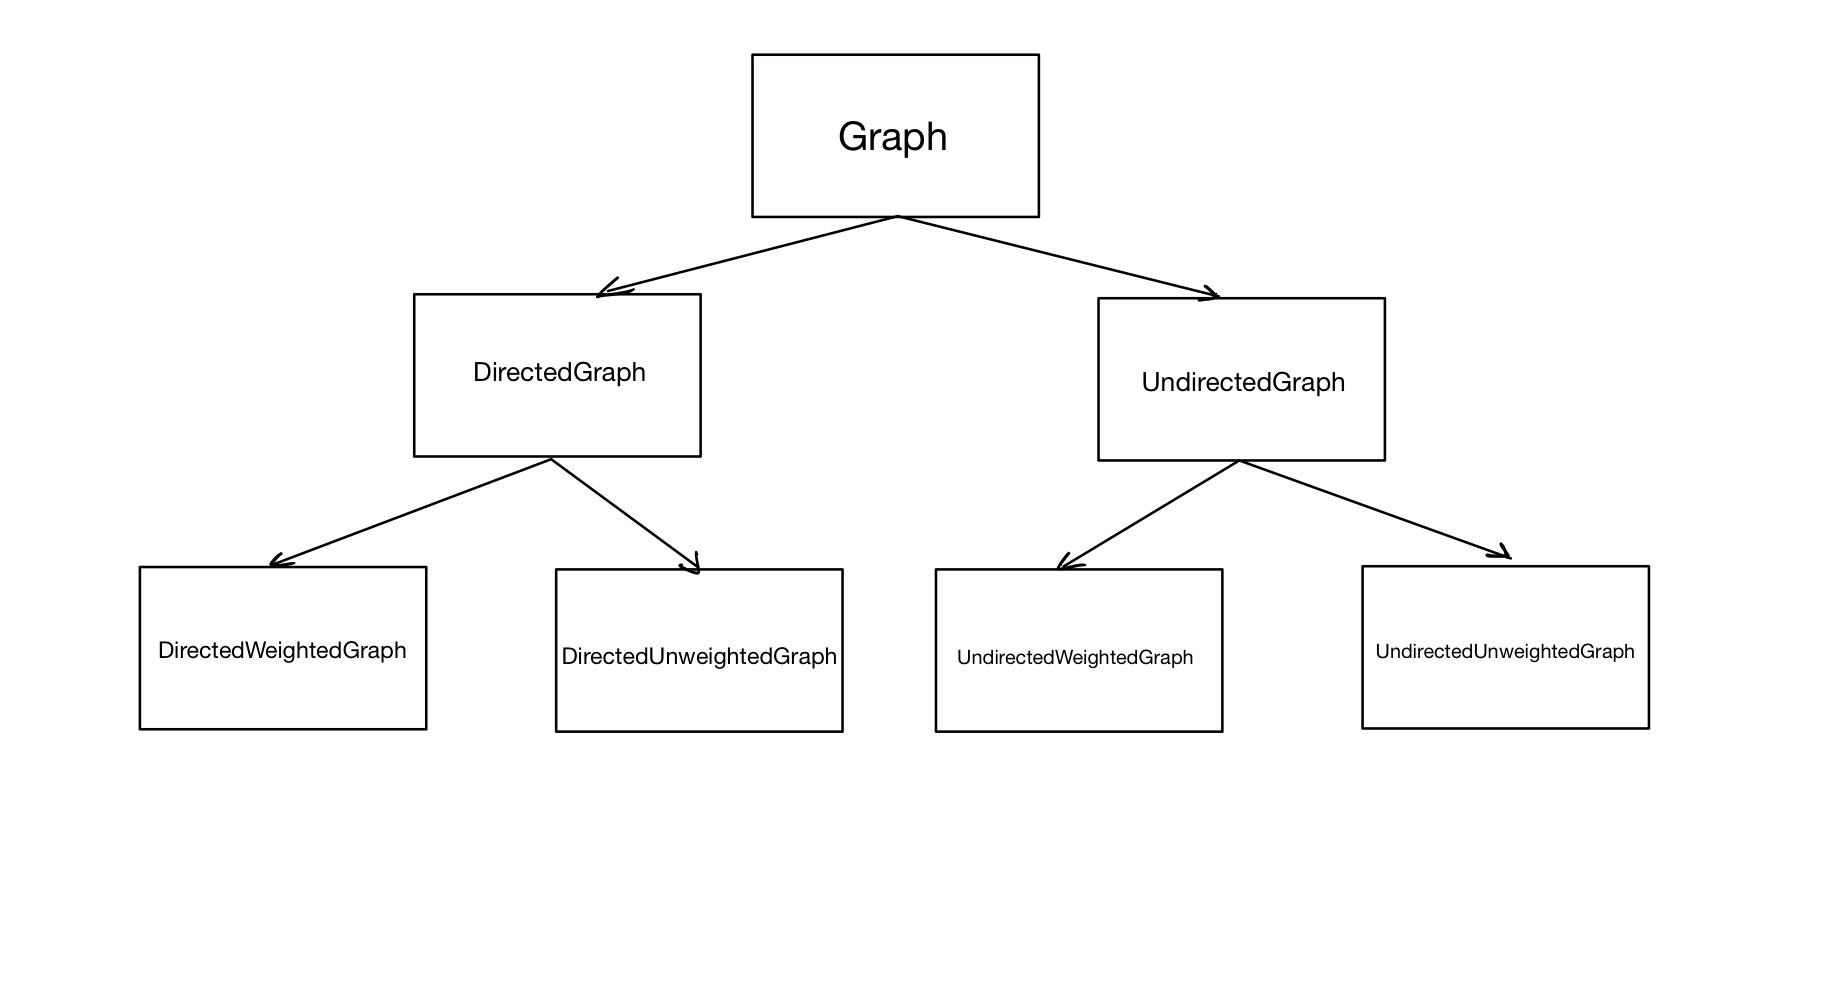
\includegraphics[width=160mm]{1_ierarx.png}
\end{center}
\bigskip

\section{Проверка графа на корректность}

Стоит сразу сказать, что все методы могут работать с графом
только в том случае, если он корректно создан, поэтому почти во все
методы встроена проверка на корректность графа. (По умолчанию, при создании объекта,
граф считается корректным)
\bigskip

Поле, которое показывает корректность или некорректность графа имеет следующий вид:
\bigskip

\lstinputlisting{2_isNormal.java}
\bigskip

Это поле может быть изменено только в методе setGraph и readGraphFromFile. Очевидно,
что в случае успешного выполнения эти методы присвоят полю isNormal значение true,
в случае возникновении ошибки (если до этого граф не был создан), полю будет
присвоено значение false.

\section{Создание графа (конструкторы)}

\subsection{Создание пустого графа}

Пустой граф создаётся простой инициализацией списка смежноси:
\bigskip

\lstinputlisting{3_empty_graph.java}
\bigskip

Этот конструктор с точностью до имени одинаков для остальных
видов графов.

\subsection{Создание графа по списку смежности}

Для создания графа по списку смежности конструктору передаётся
список смежности, который сразуже передаётся в метод setGraph,
в котором уже и будет решено, будет создан граф по переданному списку смежности
или нет.
\bigskip

\lstinputlisting{4_graph_by_linked_list.java}
\bigskip

\subsection{Создание графа по списку смежности из текстового файла}

Для создания графа по списку смежности, который хранится в текстовом файле,
нужно передать конструктору строку, являющуюся абсолютным путём к данному
текстовому файлу. Далее этот путь будет передам методу readFromFile для чтения
из файлай списка смежности и последующей отправки полученного списка методу
setGraph.
\bigskip

\lstinputlisting{5_graph_by_file.java}
\bigskip

\subsection{Создание графа с помощью другого графа}

Для создание графа, по уже созданному графу необходимо передать
в конструктор граф такого же типа, что мы и хотим создать. После этого
переданный граф будет проверен на корректность, и, в случае успешного
прохождения проверки, будет создана копия списка смежности и присвоена
списку смежности создаваемого графа, а его статус будет заменён на корректный.
\bigskip

\lstinputlisting{6_graph_by_graph.java}
\bigskip

\section{Задание графа (setGraph)}

Задать граф можно с помощью метода setGraph. На вход он принимает
список смежности, анлизирует его, и, если переданный список задан
корректно, присваивает новое значение списку смежности графа.
\bigskip

Анализ списка смежности на корректность проходит следующим образом:
проходимся по списку смежных вершин каждой вершины и проверяем
наличие связей с несущесвующими вершинами, если такая связь есть,
то завершаем проверку и оставляем граф в прежнем состоянии.
\bigskip

В случае взвешенного графа ещё проверяется наличие веса у связи,
то есть присутствует ли знак - после имени смежной вершины и есть ли
после него хоть 1 символ.
\bigskip

Пример некорректного списка смежности невзвешенного графа:
\smallskip

Пусть полный граф имеет вершины A, B и C. Тогда некорректный список
смежности может иметь вид:\\*
A:A B C\\*
B:A B C\\*
C:A B C Z\\

где Z~--- связь с несуществующей вершиной.
\bigskip

Пример некорректного списка смежности взвешенного графа:
\smallskip

Пусть полный граф имеет вершины A, B и C и вес связи любой равен 1.
Тогда некорректный список смежности может иметь вид:\\*
A:A-1 B-1 C-1\\*
B:A B-1 C-1\\*
C:A- B-1 C-1\\

где связи A и A- некорректны.
\bigskip

Реализация метода setGraph для взвешенного ориентированного графа
(для остальных видов графа данный метод реализуется схожим образом):
\bigskip

\lstinputlisting{7_setGraph.java}
\bigskip

\section{Считывание графа из файла}

Считывание и последующие задание графа из файла реализует метод
readGraphFromFile.
\bigskip

На вход метод получает абсолютный путь до считываемого файла и действует
следующим образом:

\begin{enumerate}
  \item {открывает файл. в случае успешного открытия переходит к пункту 3, в
  противном случае переходит к пункту 2;}
  \item {выводится сообщение о соответствующей ошибке и, если граф не был создан, переводит граф
  в состояние некорректности;}
  \item {создаётся пустой список смежности, после совершается переход к пункту 4;}
  \item {если файл не пустой, то считываем 1 строку и переходим к пункту 5, иначе возвращаем список смежности;}
  \item {если в строке присутствует символ : , то разбиваем считанную строку на вершину и список смежных с ней вершин, затем добавляем
  вершину и список в список смежности и переходим к пункту 4. если в строке символ : отсутствует, то переходим к пункту 2.}
\end{enumerate}
\bigskip

Реализация метода (одна на все виды графов):
\bigskip

\lstinputlisting{8_readFromFile.java}
\bigskip

\section{Основные методы работы с графом}

\subsection{Добавление вершины (addVertex)}

За добавление вершины в граф отвечает метод addVertex.
Он принимает имя вершины (строка) и список смежных
с ней вершин (массив строк).
\bigskip

Перед добавлением в граф поэтапно производятся следующие
проверки:

\begin{enumerate}
  \item {Граф проверяется на корректность. Если проверка прошла успешно,
  то переходим к пункту 3, иначе переходим к пункту 2;}
  \item {Выводим сообщение о соответствующей ошибке и завершаем работу метода;}
  \item {Проверяется наличие в графе добавляемой вершины, если она уже есть,
  то переходим к пункту 2, иначе переходим к пункту 4;}
  \item {Проверяем правильность списка смежных вершин: указаны связи только с
  существующими вершинами, если граф взвешенный, то веса заданы правильно. Если проверка прошла успешно,
  то переходим к пункту 5, иначе переходим к пункту 2;}
  \item {Добавляем вершину и список смежных с ней вершин в список смежности графа и завершаем
  работу метода (если граф неориентированный, то переходим к пункту 6);}
  \item {Добавляем в связи вершин из списка смежности вершин новую вершину, после чего
  завершаем работу метода.}
\end{enumerate}

Реализация метода для неориентированного смежного графа (данный метод реализуется
аналогично для других видов графа с точностью до пукнтов 4 и 6):
\bigskip

\lstinputlisting{9_addVertex.java}
\bigskip

\subsection{Удаление вершины (delVertex)}

За удаление вершины из графа отвечает метод
delVertex. Входными данными для него является только
имя удаляемой вершины (строка).
\bigskip

\textbf{Метод работает по следующему алгоритму:}

\begin{enumerate}
  \item {Граф проверяется на корректность. Если проверка прошла успешно,
  то переходим к пункту 3, иначе переходим к пункту 2;}
  \item {Выводим сообщение о соответствующей ошибке и завершаем работу метода;}
  \item {Проверяется наличие в графе удаляемой вершины, если вершина отсутствует,
  то переходим к пункту 2, иначе переходим к пункту 4;}
  \item {Удаляем связи с удаляемой вершиной из списков смежных вершин остальных вершин и
  переходим к пункту 5;}
  \item {Удаляем вершину из графа и завершаем работу метода.}
\end{enumerate}

Реализация метода для неориентированного взвешенного графа (реализация для остальных
видов графов аналогична):
\bigskip

\lstinputlisting{10_delVertex.java}
\bigskip

\subsection{Добавление связи между вершинами (addEdge)}

За добавление связи между вершинами отвечает метод
addEdge. Он принимает на вход имя вершины, в список смежных вершин
которой будет добавлена новая связь, и название новой связи (если
граф взвешенный, то указывается ещё и вес связи).
\bigskip

\textbf{Метод работает по следующему алгоритму:}

\begin{enumerate}
  \item {Граф проверяется на корректность. Если проверка прошла успешно,
  то переходим к пункту 3, иначе переходим к пункту 2;}
  \item {Выводим сообщение о соответствующей ошибке и завершаем работу метода;}
  \item {Проверяется наличие вершины, в которую будет дабавлена связь. Если вершина
  присутствует, то переходим к пункту 4, иначе переходим к пункту 2;}
  \item {Проверяем корректность связи: указана связь с существующей вершиной,
  вес связи корректен. Если проверка прошла, то переходим к пункту 5, иначе
  переходим к пукнту 2;}
  \item {Добавляем в список смежных вершин вершины новую связь и завершаем работу метода (если
  граф неориентированный, то продолжаем работу метода и переходим к пункту 6);}
  \item {В список смежных вершин вершины, с которой указана новая связь, добавляем
  связь с вершиной, из которой связь выходит, и завершаем работу метода.}
\end{enumerate}

Реализация метода для неориентированного взвешенного графа (для остальных видов графов
метод реализуется аналогично с точностью до пункта 6):
\bigskip

\lstinputlisting{11_addEdge.java}
\bigskip

\subsection{Удаление связи между вершинами (delEdge)}

За удаление связи между вершинами отвечает метод
delEdge. Он принимает на вход имя вершины, из списка смежных вершин
которой будет удалена связь, и удаляемой связи (если
граф взвешенный, то указывается ещё и вес связи).
\bigskip

\textbf{Метод работает по следующему алгоритму:}

\begin{enumerate}
  \item {Граф проверяется на корректность. Если проверка прошла успешно,
  то переходим к пункту 3, иначе переходим к пункту 2;}
  \item {Выводим сообщение о соответствующей ошибке и завершаем работу метода;}
  \item {Проверяется наличие вершины, для которой будет удалена связь. Если вершина
  присутствует, то переходим к пункту 4, иначе переходим к пункту 2;}
  \item {Проверяем наличие связи. Если связь присутствует, то переходим к пункту 5,
  иначе переходим к пункту 2;}
  \item {Удаляем связь из списка смежных вершин переданной вершины и завершаем работу метода
  (если граф неориентированный, то продолжаем работу метода и переходим к пункту 6);}
  \item {Из списка смежных вершин вершины, с которой указана удаляемая связь, удаляем переданную
  связь и завершаем работу метода.}
\end{enumerate}

Реализация метода для неориентированного взвешенного графа (для остальных видов графов
метод реализуется аналогично с точностью до пункта 6):
\bigskip

\lstinputlisting{12_delEdge.java}
\bigskip

\subsection{Получение списка смежности графа (getGraph)}

За получение списка смежности графа отвечает метод getGraph.
\bigskip

\textbf{Метод работает по следующему алгоритму:}

\begin{enumerate}
  \item {Граф проверяется на корректность. Если проверка прошла успешно,
  то переходим к пункту 3, иначе переходим к пункту 2;}
  \item {Выводим сообщение о соответствующей ошибке и завершаем работу метода;}
  \item {Формируется и возвращается копия списка смежности графа, после чего
  метод завершает свою работу.}
\end{enumerate}

Реализация метода для всех видов графа:
\bigskip

\lstinputlisting{14_getGraph.java}
\bigskip

\subsection{Вывод графа в консоль (printGraph)}

За вывод графа в консоль отвечает метод printGraph.
\bigskip

\textbf{Метод работает по следующему алгоритму:}

\begin{enumerate}
  \item {Граф проверяется на корректность. Если проверка прошла успешно,
  то переходим к пункту 3, иначе переходим к пункту 2;}
  \item {Выводим сообщение о соответствующей ошибке и завершаем работу метода;}
  \item {С помощью 2 вложенных циклов граф последовательно выводится в консоль в
  формате пользовательского представления, после чего работа метода завершается.}
\end{enumerate}

Реализация метода для всех видов графа:
\bigskip

\lstinputlisting{15_printGraph.java}
\bigskip

\section{Задания}

\subsection{Вывод графа в файл}

Вся реализация заключена в методе printToFile. Метод
просто последовательно выводит в файл список смежности графа:
\bigskip

Реализация метода:
\bigskip

\lstinputlisting{33_printGraphToFile.java}
\bigskip

\subsection{Работа с консолью}

Вся работа с консолью реализуется с помощью класса: WorkWithConsole.
В нём метод work и отвечает за реализацию общения пользователя с программой,
а метод help выводит всю информацию, которая необходима пользователю, чтобы
разобраться как программа работает.
\bigskip

\lstinputlisting{34_workWithConsole.java}
\bigskip

\subsection{Задание 1 вариант 6}

Условие задания: Вывести все висячие вершины графа (степени 1).
\bigskip

За реализацию задания отвечают методы: vertexDegree, hangingVertices,
printHangingVertices, outVertexDegree, inVertexDegree. Расссмотрим
каждый из них в отдельности, а потом рассмотрим общий алгоритм решения.
\bigskip

Метод inVertexDegree служит для получения входящей степени вершины.
На вход он принимает имя вершины (строка).
\smallskip

\textbf{Метод работает по следующему алгоритму:}

\begin{enumerate}
  \item {Граф проверяется на корректность. Если проверка прошла успешно,
  то переходим к пункту 3, иначе переходим к пункту 2;}
  \item {Выводим сообщение о соответствующей ошибке и завершаем работу метода;}
  \item {Перебираются все вершины графа и проверяеся наличие связи с переданной в
  метод вершины (её наличие в списке смежных веришин). Если вершина присутствует, и
  текущая просматриваеемая вершина не равна вершине, для которой вычисляется входящая степень,
  то увеличивается входящая степень на 1. После того как все вершины пройдены метод возвращает
  полученное значение и завершает свою работу.}
\end{enumerate}

Реализация метода:
\smallskip

\lstinputlisting{16_inVertexDegree.java}
\bigskip

Метод outVertexDegree служит для получения исходящей степени вершины. На вход
он принимает имя вершины (строка).
\smallskip

\textbf{Метод работает по следующему алгоритму:}

\begin{enumerate}
  \item {Граф проверяется на корректность. Если проверка прошла успешно,
  то переходим к пункту 3, иначе переходим к пункту 2;}
  \item {Выводим сообщение о соответствующей ошибке и завершаем работу метода;}
  \item {Вычисляется размер списка смежных вершин переданной вершины и возвращается
  в качестве результата, после чего метод завершает свою работу.}
\end{enumerate}

Реализация метода:
\smallskip

\lstinputlisting{17_outVertexDegree.java}
\bigskip

Метод vertexDegree отвечает за вычисление степени вершины графа.
На вход он принимает имя вершины.
\smallskip

\textbf{Метод работает по следующему алгоритму:}

\begin{enumerate}
  \item {Граф проверяется на корректность. Если проверка прошла успешно,
  то переходим к пункту 3, иначе переходим к пункту 2;}
  \item {Выводим сообщение о соответствующей ошибке и завершаем работу метода;}
  \item {В случае ориентированного графа вычисляются входящая и исходящая степени
  вершины после чего в качестве ответа выдаётся их сумма. Если граф неориентированный,
  то ыычисляется размер списка смежных вершин переданной вершины и возвращается
  в качестве результата.}
\end{enumerate}

Реализация метода для ориентированных графов:
\smallskip

\lstinputlisting{18_vertexDegree.java}
\smallskip

Реализация метода для неориентированных графов:
\smallskip

\lstinputlisting{19_vertexDegree.java}
\bigskip

Метод hangingVertices отвечает за вычисление списка висячих
вершин.
\smallskip

\textbf{Метод работает по следующему алгоритму:}
\smallskip

\begin{enumerate}
  \item {Граф проверяется на корректность. Если проверка прошла успешно,
  то переходим к пункту 3, иначе переходим к пункту 2;}
  \item {Выводим сообщение о соответствующей ошибке и завершаем работу метода;}
  \item {Перебираются все вершины графа и для каждой перебираемой вершины вычисляется её
  степень. Если сетепень вершины равна 1, то её имя добавляется в список висячих вершин.
  Когда все веершины перебраны метод возвращает вычисленный список и завершает свою работу.}
\end{enumerate}

Реализация метода:
\smallskip

Метод printHangingVertices отвечает за вывод
висячих вершин графа.
\smallskip

\textbf{Метод работает по следующему алгоритму:}

\begin{enumerate}
  \item {Граф проверяется на корректность. Если проверка прошла успешно,
  то переходим к пункту 3, иначе переходим к пункту 2;}
  \item {Выводим сообщение о соответствующей ошибке и завершаем работу метода;}
  \item {Вычисляется список висячих вершин графа, после чего его содержимое
  последовательно выводится в консоль, затем метод завершает свою работу.}
\end{enumerate}

\lstinputlisting{21_printHangingVertices.java}
\bigskip

\subsection{Задание 2 вариант 18}

Условие задания: Определить, существует ли вершина, в которую есть дуга из вершины u, но нет из v. Вывести такую вершину.
\bigskip

За реализацию задания отвечают методы: fromUAndNotFromV и printFromUAndNotV.
\bigskip

Метод fromUAndNotFromV отвечает за вычисление вершины, удовлетворяющей условию задания.
На вход он принимает вершину u (строка) и v (строка).
\smallskip

\textbf{Метод работает по следующему алгоритму:}

\begin{enumerate}
  \item {Граф проверяется на корректность. Если проверка прошла успешно,
  то переходим к пункту 3, иначе переходим к пункту 2;}
  \item {Выводим сообщение о соответствующей ошибке и завершаем работу метода;}
  \item {Проверяется наличие в графе вершины u. Если вершина присутствует, то переходим
  к пункту 4, иначе переходим к пункту 2;}
  \item {Проверяется наличие в графе вершины v. Если вершина присутствует, то переходим
  к пункту 5, иначе переходим к пункту 2;}
  \item {Метод вычисляет разность списков смежных вершин вершин u и v и возвращает
  в качестве результата первую вершины из полученной разности, после чего завершает свою работу.}
\end{enumerate}

Реализация метода для взвешенных графов (для невзвешенных графов реализация
метода аналогична, но в ней будет отсутствовать часть с отсечением веса связи):
\smallskip

\lstinputlisting{22_fromUAndNotFromV.java}
\bigskip

Метод printFromUAndNotFromV отвечает за вывод вершины, удовлетворяющей условию задания.
\smallskip

\textbf{Метод работает по следующему алгоритму:}

\begin{enumerate}
  \item {Граф проверяется на корректность. Если проверка прошла успешно,
  то переходим к пункту 3, иначе переходим к пункту 2;}
  \item {Выводим сообщение о соответствующей ошибке и завершаем работу метода;}
  \item {Проверяется наличие в графе вершины u. Если вершина присутствует, то переходим
  к пункту 4, иначе переходим к пункту 2;}
  \item {Проверяется наличие в графе вершины v. Если вершина присутствует, то переходим
  к пункту 5, иначе переходим к пункту 2;}
  \item {Метод вычисляет вершину, удовлетворяющую условию задания и выводит её,
  после чего завершает свою работу.}
\end{enumerate}

Реализация метода:
\smallskip

\lstinputlisting{23_printFromUAndNotFromV.java}
\bigskip

\subsection{Задание 3 вариант 6}

Условие задания: Построить граф, полученный из исходного удалением висячих вершин.
\bigskip

За реализацию задания отвечает метод delHangingVertices.
\bigskip

\textbf{Метод работает по следующему алгоритму:}

\begin{enumerate}
  \item {Граф проверяется на корректность. Если проверка прошла успешно,
  то переходим к пункту 3, иначе переходим к пункту 2;}
  \item {Выводим сообщение о соответствующей ошибке и завершаем работу метода;}
  \item {Вычисляет список висячих вершин графа, затем последовательно удаляет
  все входящие в список вершины с помощью метода delVertex.}
\end{enumerate}

Реализация метода:
\bigskip

\lstinputlisting{24_delHangingVertices.java}
\bigskip

\subsection{Задание 4 вариант 4}

Условие задания: Выяснить, является ли граф связным.
\bigskip

За реализацию задания отвечают методы DFS, IsConnectedGraph
и printIsConnecteGraph.
\bigskip

Метод DFS реализует обход графа в глубину. На фход он принимает вершину графа.
\smallskip

Метод работает по следующему алгоритму:

\begin{enumerate}
  \item {Граф проверяется на корректность. Если проверка прошла успешно,
  то переходим к пункту 3, иначе переходим к пункту 2;}
  \item {Выводим сообщение о соответствующей ошибке и завершаем работу метода;}
  \item {Далее от переданной вершины идёт по связям, пока они есть, если пришли в тупик,
  то возвращаемся и ищем другую связь. Если связи закончились или посещены все вершины,
  то возвращаем посещённые вершины и завершаем метод.}
\end{enumerate}

Реализация метода:
\smallskip

\lstinputlisting{25_DFS.java}
\bigskip

Метод IsConnectedGraph отвечает за проверку графа на связность,
а метод printIsConnectedGraph выводит результат этой проверки.
\smallskip

Метод работает по следубщему алгоритму:

\begin{enumerate}
  \item {Граф проверяется на корректность. Если проверка прошла успешно,
  то переходим к пункту 3, иначе переходим к пункту 2;}
  \item {Выводим сообщение о соответствующей ошибке и завершаем работу метода;}
  \item {Далее запускаем обход в глубину от каждой вершины, если хоть в 1 обходе
  не будут посещены все вершины, то граф не связный, иначе связный.
  Далее возвращаем результат проверки и завершаем метод.}


\end{enumerate}

Реализация методов:
\smallskip

\lstinputlisting{26_isConnectedGraph.java}
\bigskip

\subsection{Задание 5 вариант 26}

Условие задания: Вывести один из кратчайших (по числу дуг) путей из вершины u в вершину v.
\bigskip

За реализацию задания отвечают методы BFS, takeWay,
takeShortestPathFromUtoV и printTakeShortestPathFromUtoV
\bigskip

Методы работают следующим образом. С помощью методов takeWay
и takeShortestPathFromUtoV и алгоритма обхода в глубину вычисляется
поуровневый спуск по связям из вершины истока в вершину стока,
если на уровне найдена вершина стока, то совершается возврат по
пройденному пути, после чего метод printTakeShortestPathFromUtoV
выводи полученный путь.
\bigskip

Реализация методов:
\bigskip

\lstinputlisting{27_takeShortestPath.java}
\bigskip

\subsection{Задание 6 вариант алгоритм Краскала}

Условие задания: Дан взвешенный неориентированный граф из N вершин и M ребер. Требуется найти в нем каркас минимального веса.
\bigskip

За реализацию задания отвечает методы: krascalsAlgorithm, printKrascalsAlgorithm.
\bigskip

Они работают следующим образом: krascalsAlgorithm работает сошласно алгоритму краскала:
Сначала он строит копию текущего графа без рёбер, а затем находит в графе минимальное
неиспользованное ребро и добавляет его в копию (используется ребро, связывающее
вершины из разных компонент связности). Когда копия станет связным графом, то
возвращается эта копия и метод завершает работу.
\bigskip

Реализация методов:
\bigskip

\lstinputlisting{28_krascalsAlgorithm.java}
\bigskip

\subsection{Задание 7 варианрт 5}

Условие задания: Вывести длины кратчайших путей от u до всех остальных вершин.
\bigskip

За реализацию задания отвечают методы: dijkstrasAlgorithm и printDijkstrasAlgorithm.
\bigskip

Метод dijkstrasAlgorithm принимает на вход вершину истока и ищет длины минимальных
путей до всех вершин из вершины истока. Происходит это согласно алгоритму Дейкстры.

Сначала формирются длины путей из вершины истока до всех остальных вершин. Если
есть прямой путь (соответствующее ребро), то ставится в соответствующую ячейку
вес этого ребра, если ребра нет, то ставится бесконечность. Затем,
пока не будут пройдены все вершины, выбирается минимальное значение из построенной
таблце и строятся пути от соответствующей вершины до всех остальных +
расстояние в саму вершину. Если значение путей получаются меньше имеющихся, то
записи в таблице обновляются. Когда все вершины будут пройдены, то
список весов с именами вершин выводится в консоль.
\bigskip

Реализация методов:
\bigskip

\lstinputlisting{29_dijkstrasAlgorithm.java}
\bigskip

\subsection{Задание 8 вариант 13}

Условие задания: Вывести кратчайшие пути из вершины u до v1 и v2.
\bigskip

За реализацию задания отвечают методы: fordBelmansAlgorithm и printFordBelmansAlgorithm.
\bigskip

Методы работают следующим образом. Метод fordBelmansAlgorithm получает на вход
вершину истока и 2 вершины стока, после чего реализует алгоритм Форда"=Беллмана.

Метод составляет таблицу в которой для каждой вершины указан вес пути до неё из
истока. Сначала в таблице присутствуют конечные веса только для вершины, длина
пути до которых от вершины истока равна 1 ребру, затем алгоритм проходится по всем рёбрам и пытается
улучшить веса путей. Таких проходов алгоритм совершает n-1 раз, таким образом будут вычеслены веса путей
длиной не превышвющей максимально возможное число по рёбрам. Далее алгоритм завершает свою работу и выводит
веса путей для 2 вершин стоков.
\bigskip

Реализация методов:
\bigskip

\lstinputlisting{30_fordBelmansAlgorithm.java}
\bigskip

\subsection{Задание 9 вариант 4}

Условие задания: Вывести кратчайшие пути из вершины u до v1 и v2.
\bigskip

За реализацию задания отвечают методы: floydsAlgorithm и printFloydsAlgorithm.
\bigskip

Методы работают следующим образом. Метод floydsAlgorithm принимает вершину 
истока и две вершины стока, после чего строится матрица, в которой строки и
столбцы соответствуют вершинам. На пересичении вершин ставится в начале
вес непосредственного пути из вершину в вершину. Далее алгоритм действует
согласно алгоритму Флойда, то есть в непосредственный путь подставляет
последовательно каждую вершину графа и, если вес нового пути меньше старого,
то вес обновляется. После того, как все вершины перебраны выбираются веса
на пересечении вершины истока и вершин стоков и выводятся в консоль.
\bigskip

Реализация методов:
\bigskip

\lstinputlisting{31_floydsAlgorithm.java}
\bigskip

\subsection{Задание 10}

Условие задания: Решить задачу на нахождение максимального потока любым алгоритмом. Подготовить примеры, демонстрирующие работу алгоритма в разных случаях.
\bigskip

За реализацию задания отвечают методы: findMaxFlow и printFindMaxFlow.
Один из них реализует алгоритм Форда"=Фалкерсона и находит значение
максимального потока для заданных истока и стока. Другой выводит
это значение в консоль.
\bigskip

Реализация методов:
\bigskip

\lstinputlisting{32_findMaxFlow.java}
\bigskip

% Раздел "Заключение"
%\conclusion

%Библиографический список, составленный вручную, без использования BibTeX
%
%\begin{thebibliography}{99}
%  \bibitem{Ione} Источник 1.
%  \bibitem{Itwo} Источник 2
%\end{thebibliography}

%Библиографический список, составленный с помощью BibTeX
%
%\bibliographystyle{gost780uv}
%\bibliography{thesis}

% % При использовании biblatex вместо bibtex
%\printbibliography

% Окончание основного документа и начало приложений
% Каждая последующая секция документа будет являться приложением
\appendix

\end{document}